\chapter{Background}
In this Chapter, all technical elements needed for the understanding of the covered topics are presented.
In particular, since MC2101 is a RISC-V-based microcontroller, the RISC-V ISA is briefly described, with focus on the details of the implemented features. It is also underlined the importance of having an open-source ISA, like RISC-V, which allows the embedded system community to grow continuously, and consequently, to bring technological innovation to the IoT world without being limited by closed-source proprietary solutions. Some relevant scientific works are also presented, that are the today's state-of-the-art for system on a chip design, and all the motivations that led us to choose a new design from scratch. Regarding the RISC-V core present in the architecture, AFTAB \cite{aftab}, its design is not described in details, and only some technical characteristics will be discussed, with the purpose of being useful just for the comprehension of some architectural choices made for the microcontroller design.

\section{The RISC-V Architecture}
RISC-V is the fifth generation of the open RISC ISA design from Berkeley UC.
It was born originally to support academic research in computer architecture and today it has become the most widely used open-source instruction set in the embedded systems community. Starting from its introduction in 2010, the project has been growing continuously.
As a consequence, the number of extensions and features is now quite significant. Since it would be too much verbose explaining all details documented in the official specifications, this Section only presents the ones of interest for our system.\vspace{5mm} \newline
Any further details on RISC-V ISA can be found in the official documentation, which is comprehensively explained into two volumes that can be found in the public Github repository: \url{https://github.com/riscv/riscv-isa-manual}.

\subsection{Software Execution Environment}
Every RISC-V platform is first described by its Software Execution Environment Interface (EEI). The EEI defines: the initial state of a program running on a RISC-V core, privilege modes supported, memory and I/O accessibility and attributes, the ISA itself, the handling mode for any interrupt and exception including environment calls.
An example of EEI implementation can be a RISC-V operating system that manages multiple user-level applications controlling their accesses to physical memory through a virtual memory interface.
Regarding our RISC-V machine, since the core is not sufficiently equipped to run an operating system yet, it can be considered a bare-metal platform where all programs have full access to the physical address space.

\subsection{Instruction Set Architecture}
RISC-V has a modular design: the ISA consists of a base integer set of instructions, that must be included in every machine, plus a wide number of optional standard extensions.
The base integer ISA implements a minimal set of instructions that are enough for building up a simplified computer with full software support by themselves, including general-purpose compilers, linkers, and assemblers.
In particular, there are four groups of base ISA available:
\begin{itemize}
\item \textbf{RV32I} \& \textbf{RV64I}: two primary integer variants, with the only difference residing in their data and address parallelism (32-bit and 64-bit, respectively)
\item \textbf{RV128I}: future variant of integer set supporting 128-bit parallelism;
\item \textbf{RV32E}: a subset variant of the RV32I, implemented to support small 32-bit microcontrollers with just 16 registers.
\end{itemize}
Regarding the standard extensions, they are group of instructions developed as a result of a collective effort between industry, research community, and educational institutions to allow general-purpose software development in a wide range of applications. Extensions are a crucial key for the RISC-V flexibility, as they can be included in a specialized design, without conflict, in such a way that only the exact set of ISA features required by the application are implemented, avoiding over-architecting a particular microarchitecture style.\\
The number of standard extensions is quite large, and here are reported just some very commonly used ones:
\begin{itemize}
\item \textbf{"M" extension \textbullet Integer Multiplication and Division} \\ Adds instructions to multiply and divide values held in integer registers.
\item \textbf{"A" extension \textbullet Atomic Instructions} \\ Adds instructions that atomically read, modify and write memory locations for inter-processor synchronization.
\item \textbf{"F" extension \textbullet Single-Precision Floating-Point} \\ Adds floating-point registers, single precision computational instructions as well as load and stores instructions.
\item \textbf{"D" extension \textbullet Double-Precision Floating-Point} \\ Variant of the "F" extension for double precision arithmetic.
\item \textbf{"C" extension \textbullet Compressed Instructions} \\ Provides 16-bit forms of common instructions.
\end{itemize}
The combination of all the previous standard extensions plus a base integer is commonly known as the "G" extension, and together with the supervisor instructions implemented in the "S" extension defines all instructions needed to fully support a general-purpose operating system.

\subsection{Implemented Extensions}
Here is presented the set of instructions currently implemented in MC2101. The ISA currently includes the RV32I Base Integer Set, the "M" Integer Multiplication and Division extension, and finally the "Zicsr" Control and Status Registers (CSRs) extension.\vspace{5mm} \newline
The base integer ISA \textbf{RV32I} is divided into four core instruction \emph{formats} (R, I, S, and U Type), plus two further variants (B, J) for handling immediate values.
\begin{figure}[h!]
\vspace{0.5cm}
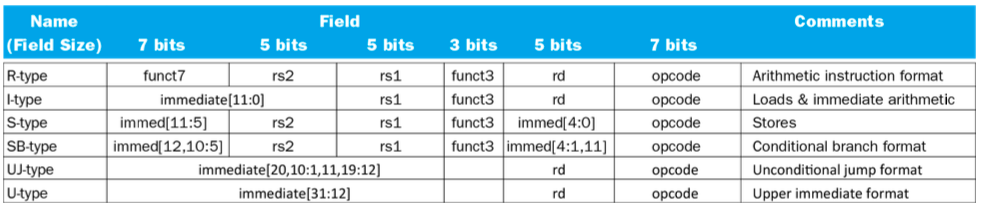
\includegraphics[width=\textwidth]{./images/rvencodings}
\caption{RISC-V ISA Encoding Formats \cite{lecture04riscv}.}
\label{fig:rve} % \ref{fig:rve}
\end{figure} 
From Figure \ref{fig:rve}, it is possible to see that the opcode, the source operands (\texttt{rs1} and \texttt{rs2}) and destination operand (\texttt{rd}) are maintained in the same bit positioning in order to reduce the decoding phase complexity.
The integer register file, used by all integer instructions, is composed of 32 general-purpose 32-bit registers.
\begin{table}
\centering
\begin{tabular}{| p{1.5cm} | p{1cm} | p{3.5cm} | p{2cm} |}
    \hline
    \textbf{Register} & \textbf{ABI Name} & \textbf{Description} & \textbf{ABI Saver}\\ \hline
    \texttt{x0} & \texttt{zero} & Hard-wired zero & / \\ \hline
    \texttt{x1} & \texttt{ra} & Return address & Caller \\ \hline
    \texttt{x2} & \texttt{sp} & Stack pointer & Callee \\ \hline
    \texttt{x3} & \texttt{gp} & Global pointer & / \\ \hline
    \texttt{x4} & \texttt{tp} & Thread pointer & / \\ \hline
    \texttt{x5} & \texttt{t0} & Temporary/alternate link register & Caller \\ \hline
    \texttt{x6-7} & \texttt{t1-2} & Temporaries & Caller \\ \hline
    \texttt{x8} & \texttt{s0/fp} & Saved register/frame pointer & Callee \\ \hline
    \texttt{x9} & \texttt{s1} & Saved register & Callee \\ \hline
    \texttt{x10-11} & \texttt{a0-1} & Function arguments/return values & Caller \\ \hline
    \texttt{x12-17} & \texttt{a2-7} & Function arguments & Caller \\ \hline
    \texttt{x18-27} & \texttt{s2-11} & Saved registers & Callee \\ \hline
    \texttt{x28-31} & \texttt{t3-6} & Temporaries & Caller \\ \hline
    \hline
\end{tabular}
\caption{RISC-V Integer Register File summary.}
\label{tab:iregfile} % \ref{tab:iregfile}
\end{table}
Table \ref{tab:iregfile} shows the registers names together with the ABI conventions. Notice that the program counter is not part of the register file itself, as the software cannot directly address it.\vspace{5mm} \newline
Part of the implemented ISA is also the Integer Multiplication and Division extension \textbf{RV32M}, which contains instructions that multiply or divide values held in two integer registers (see Table \ref{tab:iregfile}). The reason that made designers to separate multiply and divide out from the base integer is because usually multiplications and divisions operations are either infrequent or better handled by specialized accelerators. Thanks to this extension, the ISA can support multiplications, divisions, and reminder operations (No operation allows computing both Quotient and Reminder of a division).\vspace{5mm} \newline
The last extension implemented is the Control and Status Registers extension \textbf{Zicsr}, containing instructions needed to operate on CSRs registers. CSRs are a particular class of registers that can only be addressed by the Zicsr instructions and they are primarily used by privileged architecture to perform very specific tasks, e.g., handling exceptions, interrupts and traps. RISC-V ISA counts a total amount of 4096 CSRs but allow to implement just a subset of them. Our platform, for example, includes only those required for handling exceptions, interrupts, traps and for supporting User and Machine privilege levels.

\subsection{Privilege Levels}
Privilege levels are used to provide a protection mechanism, embedded in the hardware itself, between the different components of software stack, in such a way that any attempt to perform operations not permitted by the current privilege mode will rise an exception.
\begin{figure}[h!]
\centering
\vspace{0.5cm}
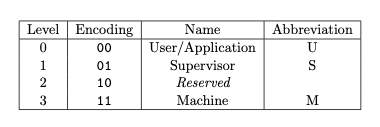
\includegraphics[scale=0.9]{./images/rvprivileges}
\caption{RISC-V Supported Privileges \cite{riscvII}.}
\label{fig:rvpri} % \ref{fig:rvpri}
\end{figure}
Figure \ref{fig:rvpri} shows all privilege modes supported by a RISC-V machine. These modes are listed in order of increasing privilege, where \emph{Machine} mode is the most privileged and \emph{User} mode being the least. All RISC-V systems must implement the \emph{M} mode, while the other are optional extensions.\\Thus, any RISC-V platform must fall in one of the following configurations, depending on the requirements:
\begin{itemize}
\item \textbf{M} \\ Simple embedded system.
\item \textbf{M, U} \\ Secure embedded system.
\item \textbf{M, S, U} \\ Systems running Unix-like operating systems.
\end{itemize}
When designing a RISC-V platform, the proper set of privileges must be carefully chosen based on the complexity of the software it will run. For instance, a small device that runs a single, \emph{thrusted} application may choose to only support \emph{Machine} mode: in this case, the application must be secure because it has full low-level access to the hardware. The modality \emph{Machine - User} is suitable for secure embedded systems. It provides a level of isolation between the application and a direct access to the hardware, by using \texttt{ecall} instruction to perform machine-level operations, that can fully and directly access the hardware. The full software stack separation is reached when the machine implements the \emph{Machine - Supervisor - User} mode. In this case the ISA is able to support a more robust system where there is an operating system working as intermediate between user and hardware.\vspace{5mm} \newline
Since our microcontroller is intended to be used as a security platform, it implements both \emph{M} and \emph{U} privileges required for a secure embedded system.
\begin{figure}[h!]
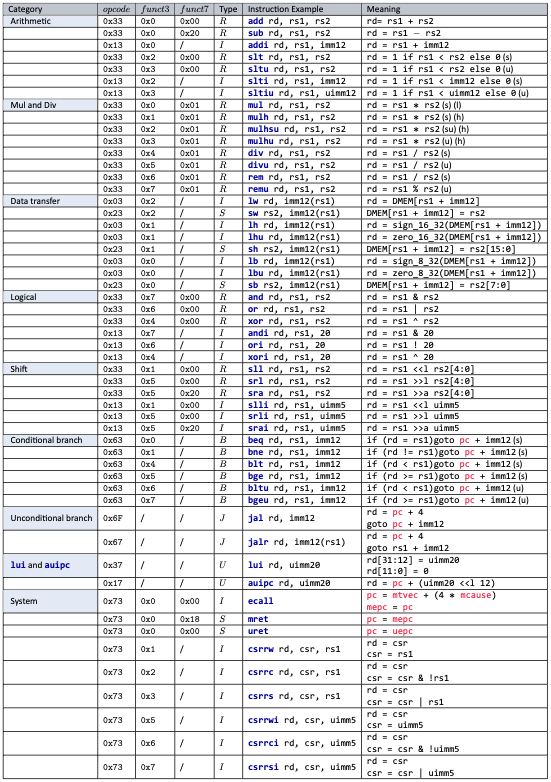
\includegraphics[scale=0.7]{./images/mc2101isa}
\caption{Implemented Instruction Set \cite{aftabManual}.}
\label{fig:mc2101i} % \ref{fig:mc2101i}
\end{figure}

\section{RISC-V Importance in IoT era}
Provided the main features of the RISC-V ISA, it should be clear the advantage that a modular architecture of this type can bring in terms of design freedom and use cases. In fact, the various extensions allow to design any kind of chip, from very small 16-bit low-power and cost-constrained microcontrollers, to extremely complex 64-bit full-featured high-performance SoCs. But why is there any need for a new instruction set architecture when there are several popular commercial ISAs available, that could be reused avoiding the significant effort and cost of porting software to a newer one?

The first reason behind the adoption of the RISC-V ISA as the standard architecture in academia and research is that all popular commercial ISAs, like x86 or ARM, are \emph{proprietary}. This means that vendors have a lucrative business in selling implementations, both in form of IP cores and silicon. Because of this, it is economically not sustainable for many companies, universities, or individuals, to develop custom designs. Another reason is that all popular commercial ISAs are massively \emph{complex}. In particular, the increasing complexity of legacy microprocessors has become profound, requiring hundreds of engineers, millions in investment, years in development, and all this complexity lead to a very inefficient and power-hungry design, for sure not suitable for IoT applications. It is therefore very difficult to fully implement one of those legacy architectures. Also, there is a little incentive to create subset ISAs, for more specialized design, because the software cannot run without being modified as well. For the aforementioned reasons, having an open source architecture like RISC-V, with tons of materials available for free, as well as a wide variety of projects going on, is a fundamental architecture that can help to overcome the barriers imposed by proprietary solutions. Among all the available open-source RISC-based ISA, RISC-V was designed to face these problems, through its modular architecture that allows to be used in any kind of applications, suitable also for educational purposes thanks to the simple base integer subset.

\begin{table}
\centering
\begin{tabular}{| p{4cm} | p{4cm} | p{4cm} | p{4cm} |}
 \hline
 \textbf{Barriers} & \textbf{Legacy ISA} & \textbf{RISC-V ISA}\\ \hline
 \hline\hline
 Complexity & 1500+ instructions, incremental ISA & 47 base instructions, modular ISA \\ 
 \hline
 Design freedom & \$\$\$ - Limited & Free - Unlimited  \\
 \hline
 License and Royalty fees & \$\$\$  & Open Source  \\
 \hline
 Design ecosystem & Moderate & Growing rapidly. Numerous extensions, numerous open cores. \\
 \hline
 Software ecosystem & Extensive & Growing rapidly \\
 \hline
\end{tabular}
\caption{Summary of RISC-V advantages with respect to Legacy ISAs \cite{riscvIntro}.}
\label{tab:legacy} % \ref{tab:legacy}
\end{table} 

The Table \ref{tab:legacy} is useful to summarize the advantages that the RISC-V ISA can offer with respect to popular commercial ISAs. These are the main reasons that allowed RISC-V to grow and become the today standard ISA used for embedded systems design in academia and research world.

It is important to underline that RISC-V is not only a revolution for hardware design in academia and research: it is also cracking a new commercial market wide open. As the IoT era keeps growing day by day, more and more companies are starting to develop their own chip, and companies that long prized for their proprietary architectures, like ARM, Intel and others, suddenly have to contend and compete with this new way of thinking and building. Therefore, it is essential that universities train engineers capable of designing efficient and reliable microarchitectures and also that the research can continue to produce innovative ideas that allow IoT technology to be widespread.

\section{State of the Art in Embedded System Design}
In this Chapter, some relevant state-of-the-art works are presented, featuring relevant scientific works related to RISC-V. As the purpose of my thesis is the design of a microcontroller, this Chapter discusses some of the most popular open-source RISC-V based SoCs, designed for energy-efficient computing. To stress again on the wide possibility that the RISC-V ISA can offer, three different types of architecture are here presented. 

The first one is the BOOM \cite{zhaosonicboom} SoC, part of the Berkeley Hardware CPUs, a very complex platform with an infrastructure usable for personal, supercomputer and warehouse-scale computers. The second example is about PicoRV32 \cite{picorv32} by Claire Wolf, a 32-bit microcontroller class RV32IMC implemented in Verilog HDL. The third and last example focuses on PULPino \cite{pulpino} from ETH Zürich and University of Bologna, which is a simple microcontroller that can be extended for being used as custom embedded DSP. The architecture of this last microcontroller has been particularly important for my thesis work, because it has been used as a reference.

\subsection{Berkeley Out of Order Machine}
The BOOM machine is a synthesizable and parameterizable open-source RV64GC RISC-V core, written in Chisel \cite{chisel}. As its name suggest, BOOM is an out-of-order processor, inspired by the MIPS R10000 \cite{491460} and the Alpha 21264 \cite{755465} processors . Created at the University of Berkeley (California) in the Berkeley Architecture Research group, its focus is to provide a high performance, synthesizable and parameterizable SoC for architecture research. This is a perfect example to underline how much degree of complexity can be reached by using RISC-V extensions.

\begin{figure}[h!]
\centering
\vspace{0.5cm}
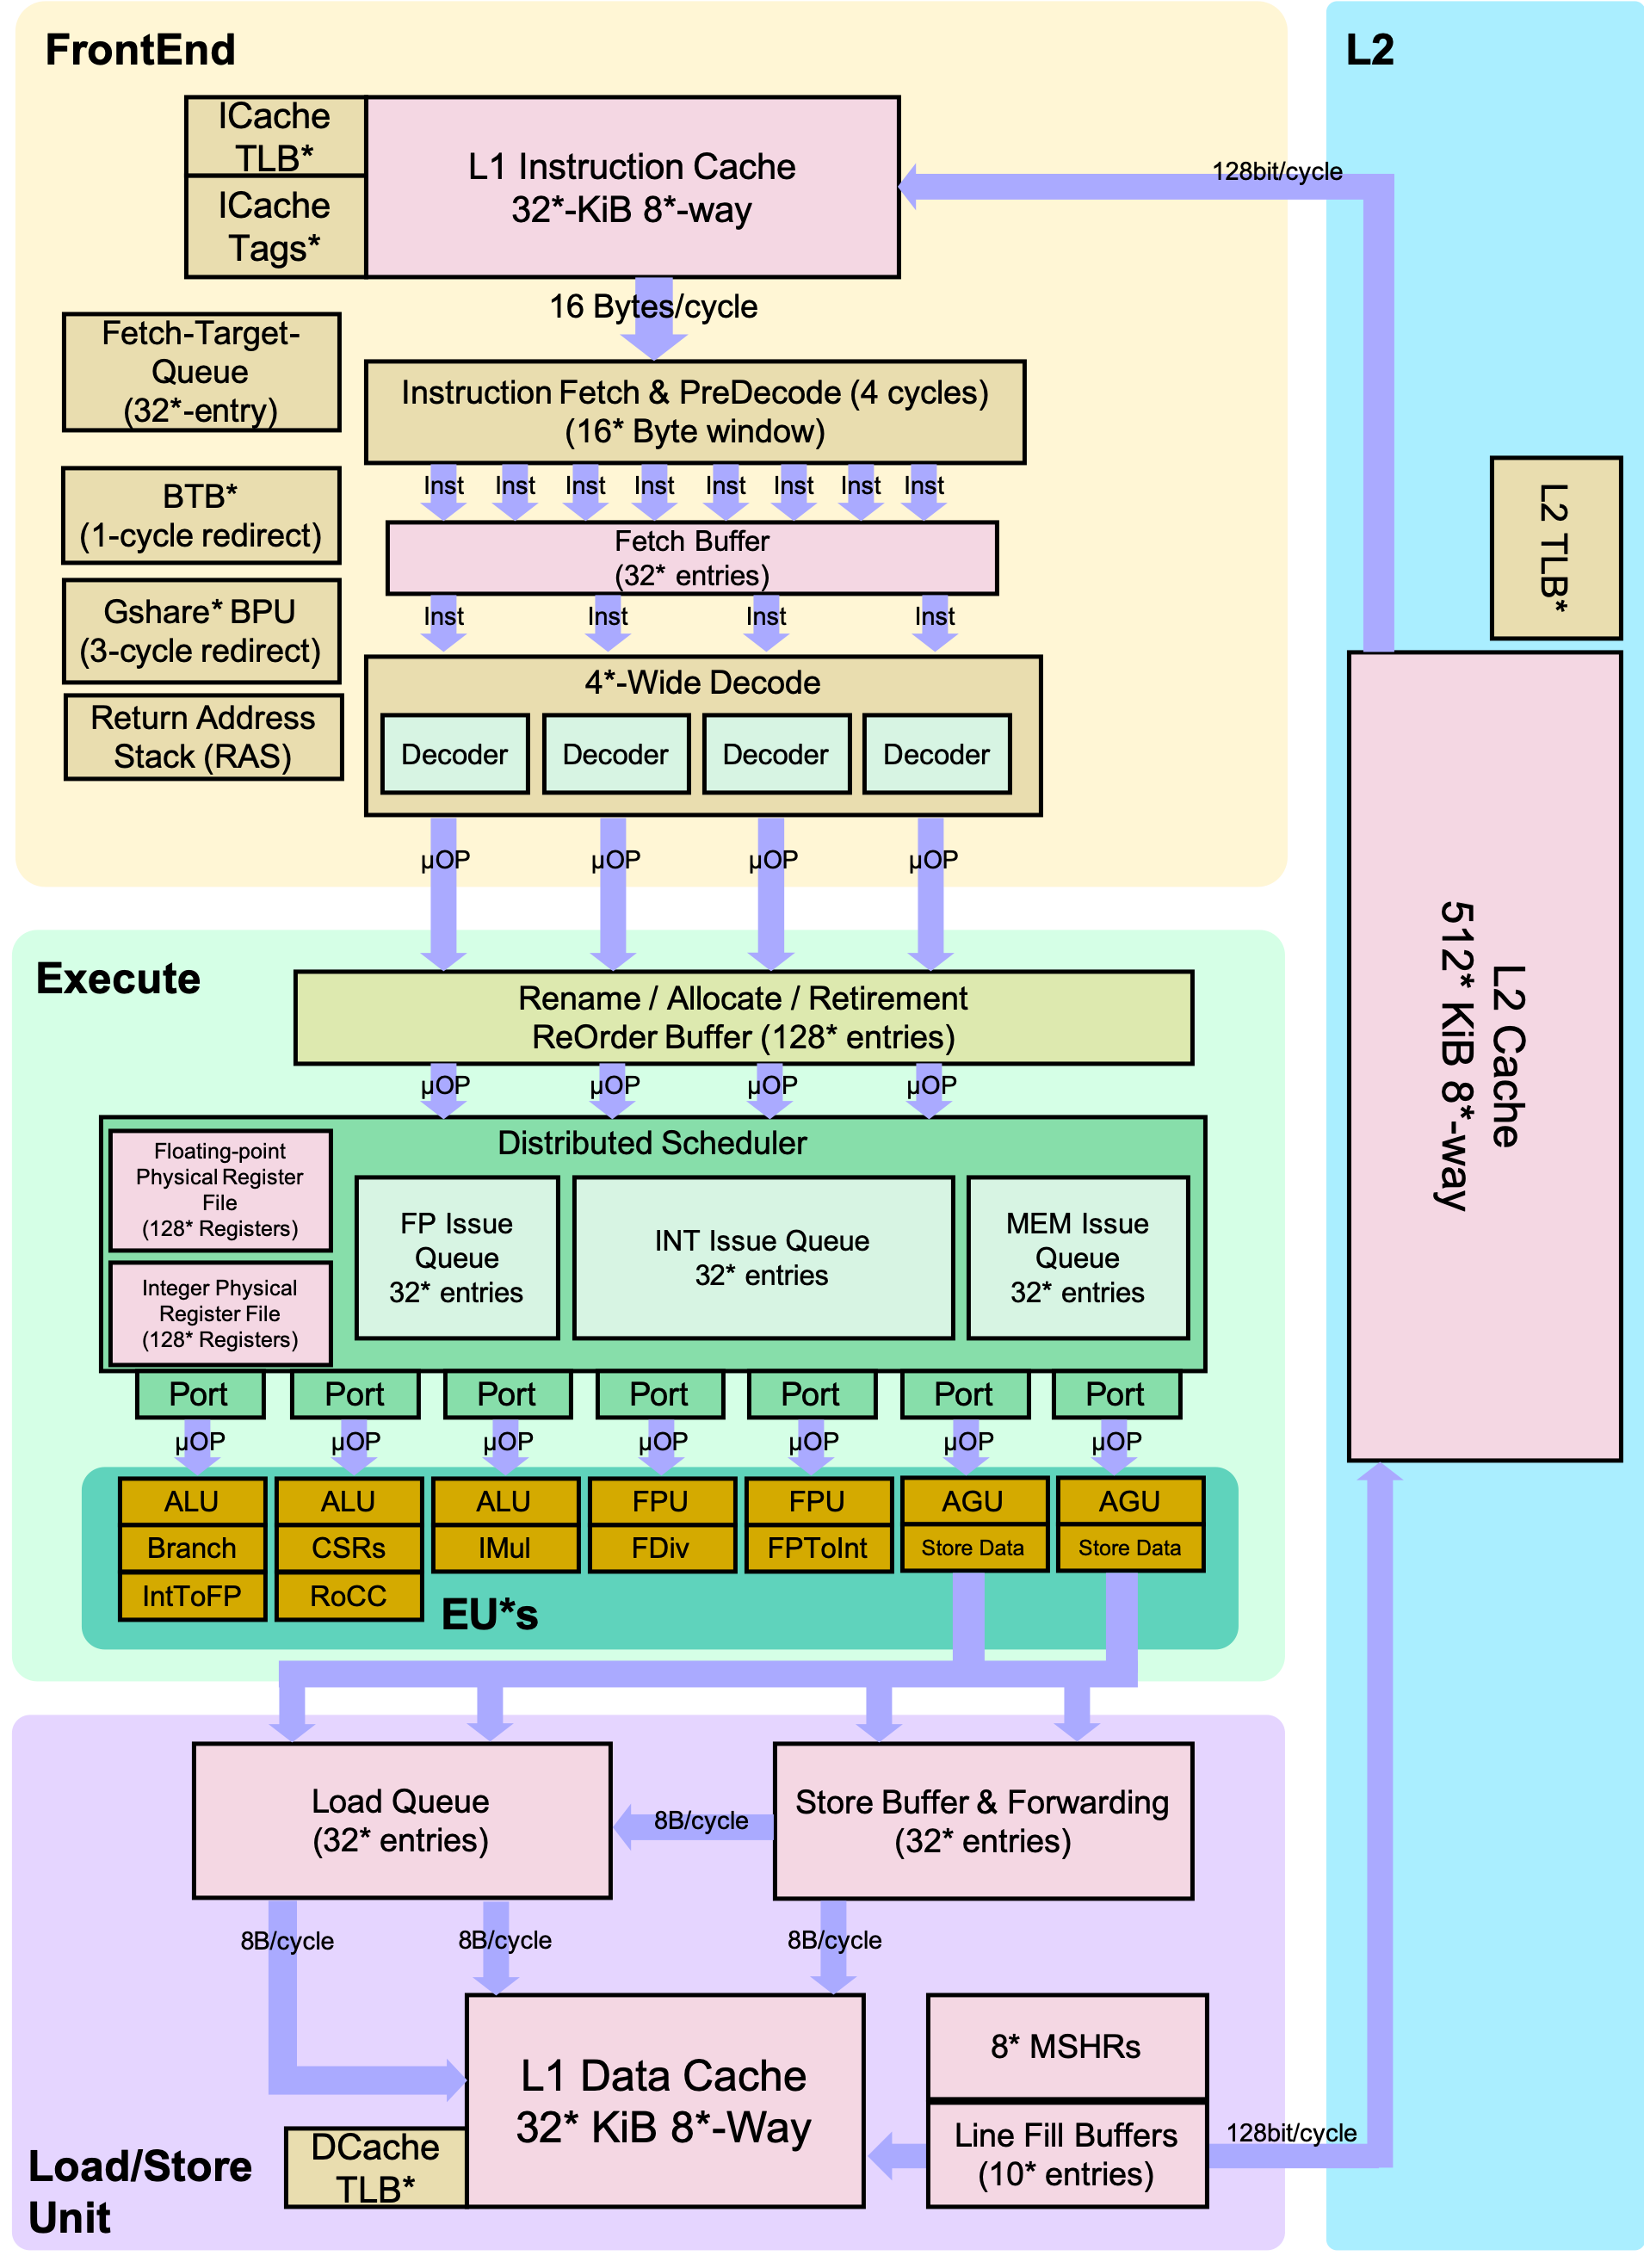
\includegraphics[scale=0.2]{./images/boom-core}
\caption{BOOM Architecture Overview \cite{zhaosonicboom}.}
\label{fig:boom} % \ref{fig:boom}
\end{figure}

From Figure \ref{fig:boom}, it is possible to distinguish the classical pipeline stages of out-of-order architectures. Conceptually, the processor implements 10 stages: \texttt{Fetch}, \texttt{Decode}, \texttt{Register Rename}, \texttt{Dispatch}, \texttt{Issue}, \texttt{Register Read}, \texttt{Execute}, \texttt{Memory}, \texttt{Writeback} and \texttt{Commit}. The architecture is then able to execute instructions in out-of-order fashion, pushing even more the throughput and performances of a standard pipeline. The fact that it also implements a 64-bit version of the standard \texttt{G} indicates this core is designed exclusively for high performance systems.

Further details can be found in the official Github repository\footnote{\url{https://github.com/riscv-boom/riscv-boom}}, where it is also possible to access at the RTL description.

\subsection{Picorv32 microcontroller}
The PicoRV32 is a microcontroller that implements the RV32IMC instruction set written in Verilog. This microcontroller can be configured in many different ways, starting from the core itself that can be configured to support the following extensions: \texttt{RV32I}, \texttt{RV32IC}, \texttt{RV32IM} and the \texttt{RV32IMC}. The architecture of the microcontroller is also available in the following configurations:

\begin{itemize}
\item \texttt{picorv32}: simplest version that implements a simple native memory interface, usable in simple environments;
\item \texttt{picorv32\_axi}: provides an AXI-4 Lite Master interface that can be easily integrated within other systems based on AXI standard bus infrastructure;
\item \texttt{picorv32\_wb}: provides a Wishbone bus master interface;
\item \texttt{picorv32\_axi\_adapter}: This core provides a bridge between the native memory interface and an AXI4 infrastructure. This implementation can be used to create custom cores that include one or more \texttt{picorv32} cores together within a compact microcontroller that internally can communicate using a native custom lightweight interface, and externally can be attached through AXI4.
\end{itemize}

It is possible to understand that this embedded system is meant to be used as auxiliary processing device in FPGA designs and ASICs. The architecture includes also a UART peripheral and a SPI Flash Controller.
Any additional information can be found in the official Github repository\footnote{\url{https://github.com/YosysHQ/picorv32}}.

\subsection{PULPino}
Developed by ETH Zurich and the University of Bologna, PULPino is a RISC-V-based single-core SoC written in SystemVerilog, which represents a small part (one core) of the Parallel Ultra-Low Power (PULP) platform designed for energy-efficient IoT parallel computing.

In Particular, the PULP SoC is a cluster that embeds a configurable number of RISC-V based cores with a design focused for being extremely low power consuming. Perfectly suited for IoT devices that requires high computational capabilities. PULPino represents a first step towards the release of the full PULP platform. In fact, PULPino inherits from its bigger brother some of the IPs and the core, focusing on ease of use and simplicity.

\begin{figure}[h!]
\centering
\vspace{0.5cm}
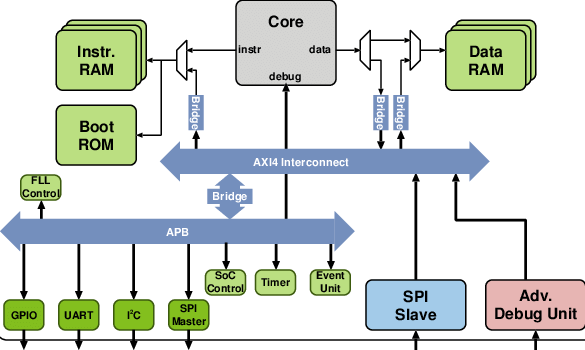
\includegraphics[scale=0.6]{./images/pulpino}
\caption{PULPino Microcontroller \cite{pulpino}.}
\label{fig:pulpino} % \ref{fig:pulpino}
\end{figure}

Figure \ref{fig:pulpino} shows the design overview of the SoC. From an architectural point of view, it is a simple single-core AMBA-based embedded system. It offers a modular design that does not include complex features like caching mechanisms, memory hierarchy or DMA. The core is directly connected to the IRAM and DRAM in a single access, no waiting manner. There is a central AXI interconnection, that interconnects the processor with the memories, allowing pipelined high-bandwidth operations. Regarding the core, the microcontroller is based on a 32-bit RISC-V architectures and can be configured to use either the \texttt{RISCY} or the \texttt{zero-riscy} core. Both developed at ETH Zürich.

\begin{figure}[h!]
\centering
\vspace{0.5cm}
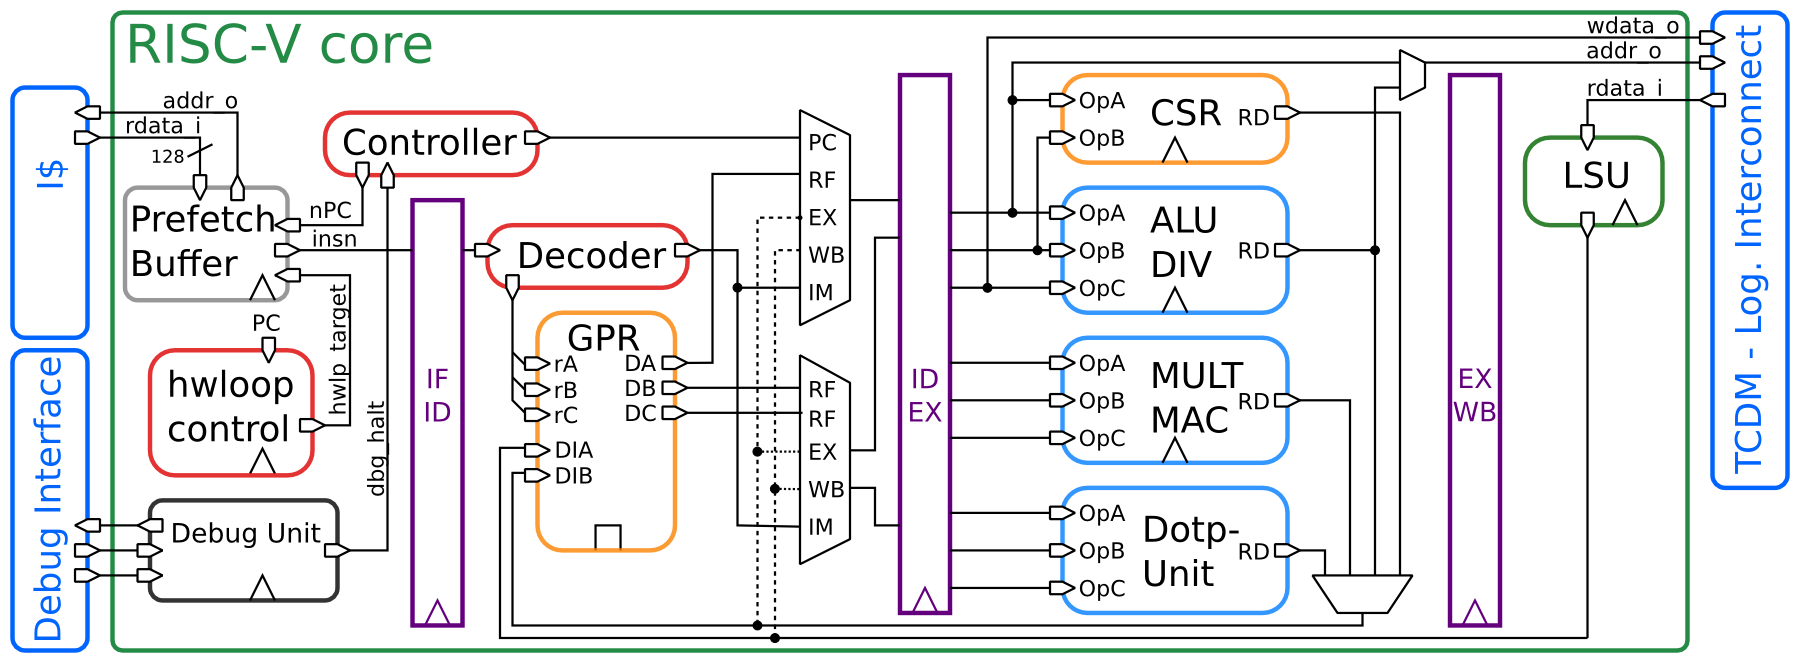
\includegraphics[scale=0.7]{./images/riscy}
\caption{RISCY core.}
\label{fig:riscy} % \ref{fig:riscy}
\end{figure}

The \texttt{RISCY} core, shown in Figure \ref{fig:riscy}, is an in-order, single-issue core with 4 pipeline stages able to guarantee an IPC close to 1. The ISA supports the base integer instruction set (RV32I), compressed instructions (RV32C), multiplication and division instruction extension (RV32M). In can also be configured to implement the RV32F extension for single-precision floating point operations. It also implements several custom ISA extensions such as hardware loops, post-incrementing load and store instructions, bit-manipulation instructions, MAC operations, fixed-point operations, packed-SIMD instructions and the dot product. All these additional features have been implemented for allowing ultra-low-power signal processing applications. Also, a subset of the 1.9 privileged instructions are supported.

\begin{figure}[h!]
\centering
\vspace{0.5cm}
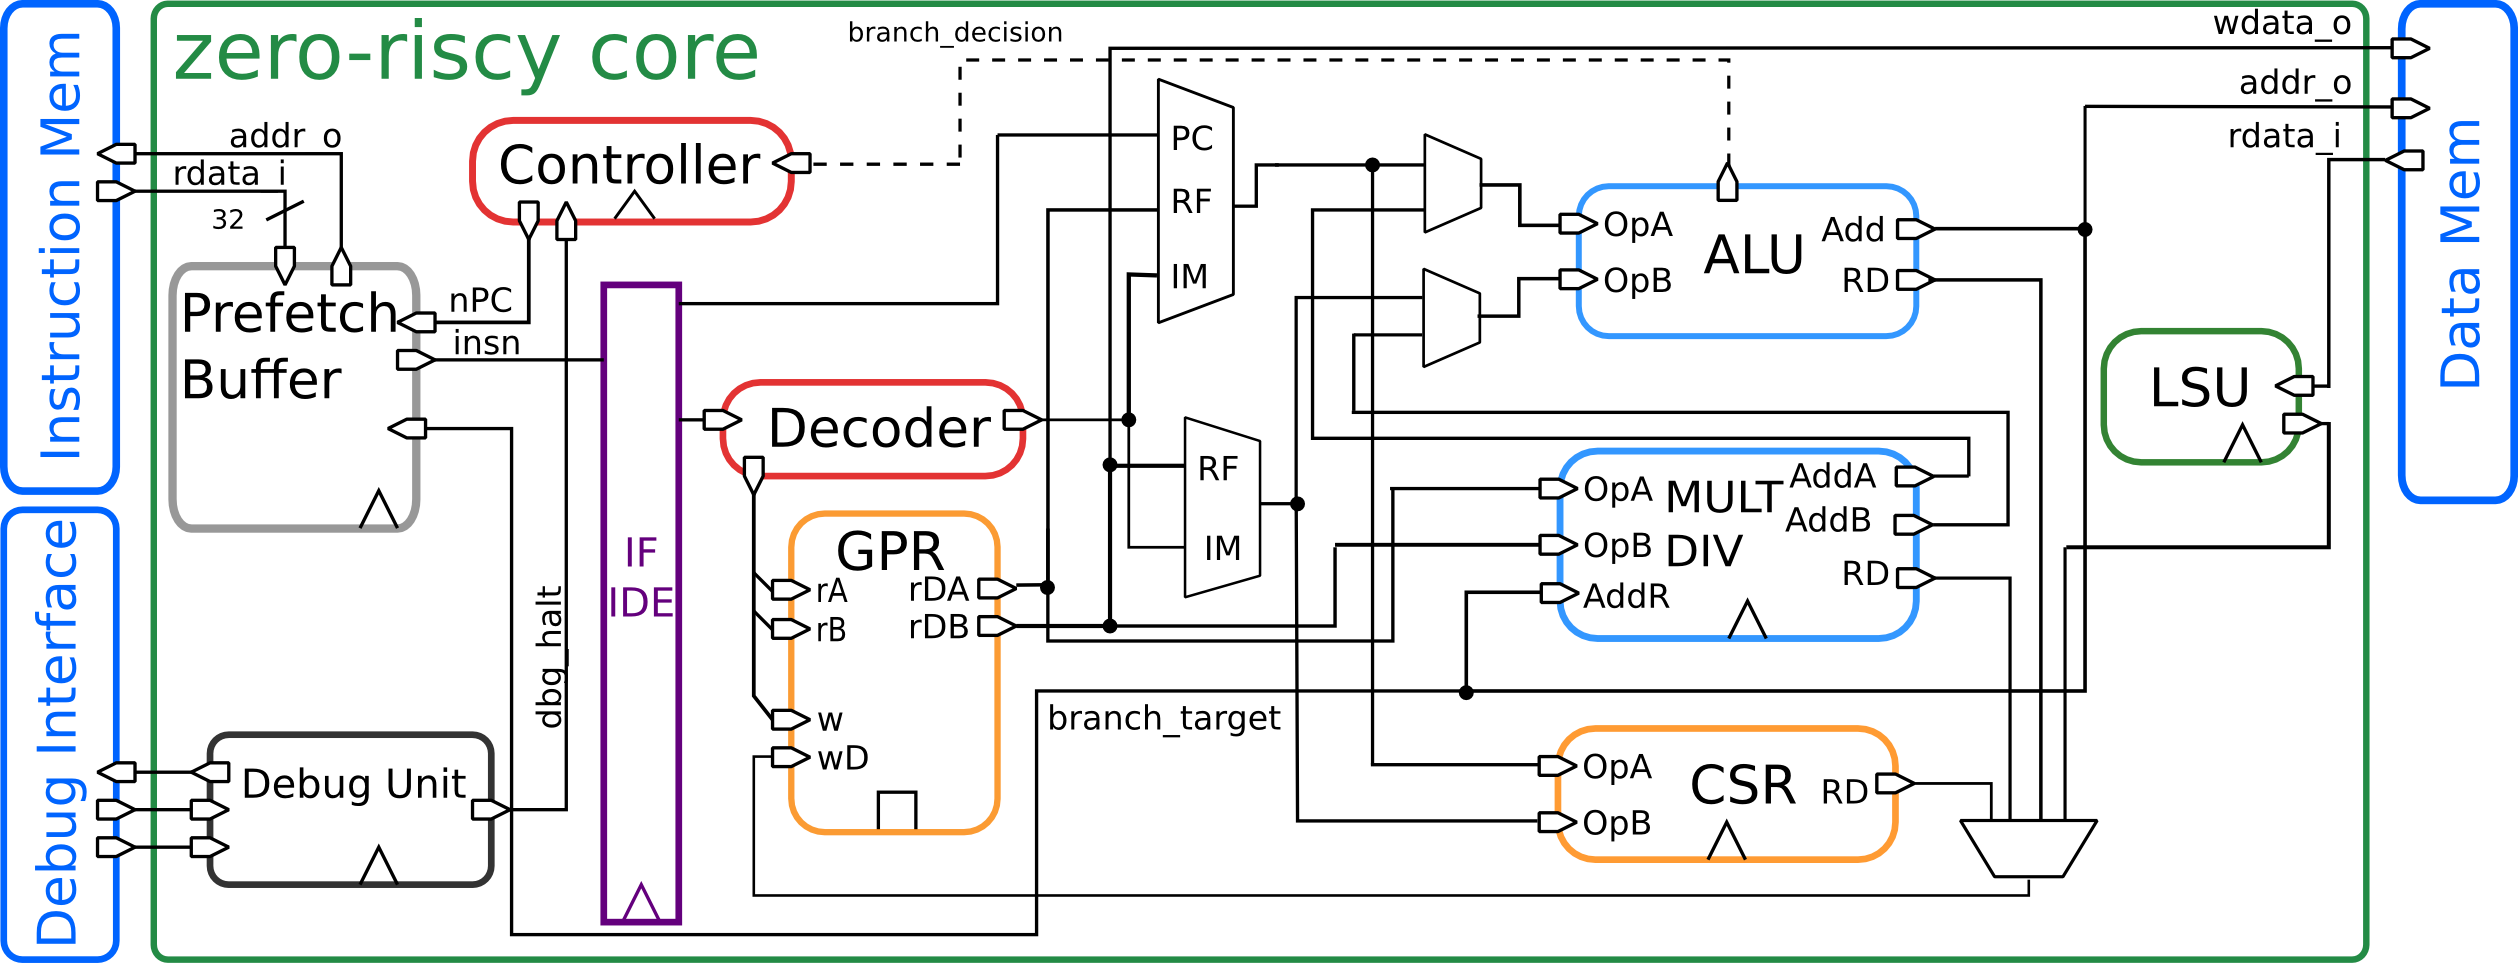
\includegraphics[scale=0.7]{./images/zeroriscy}
\caption{Zero-riscy core.}
\label{fig:zeroriscy} % \ref{fig:zeroriscy}
\end{figure}

The \texttt{Zero-riscy} core, depicted in Figure \ref{fig:zeroriscy}, is instead a much more simpler processor. Suitable for ultra-low-power ultra-low area constrained embedded systems. It is an in-order, single issue core with 2 pipeline stages supporting the RV32I, RV32C and a subset of 1.9 privileged ISA. Can also be configured to implement the RV32M and the reduced number of register extension RV32E. The architecture offers a secondary bus level that interconnects a broad set of peripherals for the communication with the outside world. Part of the implementations are also the SPI Slave and the Debug Unit, which are used to pre-load the RAMs with executable code from SPI flash and to allow access to the whole memory map via JTAG for debugging purposes.

Among all the available microarchitectures, PULPino is the one chosen to be our reference architecture. This is because it implements in a very simple and compact design all the features necessary to have a complete usable microcontroller-style platform, closer to our requirements. Also, what makes PULPino perfect for being used as a reference soft microcontroller is for sure its modular and clean design, the extensible software toolchain built around it for cross-compilation, RTL simulation and synthesis, together with a great documentation to support usage and learning.

The RTL description, as well as the entire toolchain for simulations, compilation and FPGA synthesis can be found in the official Github repository\footnote{\url{https://github.com/pulp-platform/pulpino}}.

\section{Our contribution to the RISC-V community}
Whenever an team of engineers decide to start designing a new RISC-V platform, the first possible way to act is to start from an already implemented open-source platform, like one of those seen before, where it is possible to include custom integrations and modify the existing design to fulfil the desired behaviour. The second choice would be to start a new design from scratch, by using some well known architecture as a reference. There are two factors on which the choice of the path to take is based: the first one regards the specifications and use cases of the embedded device. For instance, if the target is to design a low-power IoT device, if one wants to start from something already developed, he or she must have a soft lightweight microcontroller to customise, otherwise there is the need to start a new design from scratch. The second factor is related to the technical background of the team on HDL languages, which require a certain degree on know-how in order to develop clean and synthesizable designs. Embedded Systems engineers in Politecnico di Torino, for example, have strong expertise in VHDL, but not in SystemVerilog or Chisel HDLs, and this reflects to the students.

Regarding our RISC-V based platform MC2101, the research team that hosted me needed to have a RISC-V based architecture entirely customizable and synthesizable. The particular aim of our platform is to offer the possibility to integrate hardware security solutions and also to assess and evaluate them through software testing. Those kind of solutions first require a simple architecture that can be easily customised starting from the core itself, and then a proper toolchain for automating all the processes of RTL simulation, synthesis and compilation.

Among all the most popular solutions available in literature, the PULPino architecture mentioned before is for sure the one that comes closest to our needs. Referring again to the Figure \ref{fig:pulpino}, it is a modular design, easy to use, that includes all the set of peripherals necessary to interact with the microcontroller once synthesized on FPGA, as well as the necessary interfaces used to debug and flash the firmware on it. All these features are what is needed to test the architecture and any custom integration. Of great importance is also the \emph{software toolchain}, created with the aim of automating all the processes of synthesis, RTL simulations, and software compilation. The big problems with PULPino, common to many other RISC-V most popular open-hardwares, is that it is fully described using SystemVerilog hardware description language, which is not part of our background as computer engineers.

It was therefore mandatory to opt for our own design, developed from scratch, fully implemented in VHDL. The AFTAB processor, briefly described in the next Section, was the first step of the development.

\section{The AFTAB Processor}
AFTAB, acronym for ``A Fine Turin/Tehran Architectural Being'', is an in-order fully sequential (not pipelined) 32-bit RISC-V core, developed by the CINI Cybersecurity National Laboratory in cooperation with University of Tehran. The processor works according to the Von Neumann architecture, so there is only a single RAM containing both data and instructions.

As for the implementation details, its enough to give a high-level description of the processor, starting from its interface and going directly to the programmer's model.
\subsection{AFTAB Interfacing Ports}

\begin{figure}[h!]
\vspace{0.5cm}
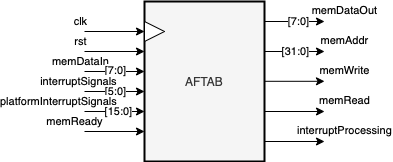
\includegraphics[scale=0.9]{./images/aftabpins}
\caption{AFTAB microprocessor interface.}
\label{fig:aftabpin} % \ref{fig:aftabpin}
\end{figure}

The core can be described as a blackbox component (Figure \ref{fig:aftabpin}), whose pins can be grouped into the Memory Interface set and the Interrupt Interface set. The Memory Interface includes these signals:

\begin{itemize}
\item \texttt{memRead} \& \texttt{memWrite}: read and write signals for the memory. Forwarded in the MC2101 bus in order to start a transaction that can target the main memory or any peripheral
\item \texttt{memReady}: fundamental signal used to stall the processor in the fetch stage. In this way, by controlling this signal, the bus infrastructure can take the necessary time to complete read and write operations;
\item \texttt{memAddr}: AFTAB address bus is 32-bit wide;
\item \texttt{memDataIn} \& \texttt{memDataOut}: two 8-bit ports that together build the data bus of the microcontroller. During load and store operations, they carry variable number of bytes per transaction (1, 2, or 4) in a sequential way, so that only one byte per clock cycle can be read or written.
\end{itemize}

As for the Interrupt Interface set, there are a total of 22 independent interrupt lines, where 16 of them are for platform use, plus an additional signal (\texttt{interruptProcessing}) indicating when the processor is in the interrupt processing states. The core is also able to handle the following hardware-level exceptions:

\begin{itemize}
\item \textbf{Illegal Instruction}: the decode phase does not recognise the opcode as a valid one;
\item \textbf{Illegal CSR instruction}: raised when there is an attempt to read or write a CSR register with an inappropriate privilege level, or when trying to access a non-existing CSR register;
\item \textbf{Instruction address misaligned}: raised after an attempt to access the instruction memory without the proper 4-bytes alignment.
\end{itemize}

For the programmer's point of view, as previously anticipated, AFTAB implements the RV32I, RV32M, and Zicsr extensions. Therefore, the instruction set supported is the one depicted in Figure \ref{fig:mc2101i}, and the registers available are the integer ones, listed in Figure \ref{tab:iregfile}.

The RTL description, as well as the entire toolchain for simulations, compilation and the manuals can be found in the official Github repository\footnote{\url{https://github.com/RHESGroup/aftab}}.